\documentclass[12pt]{beamer}
\usetheme{Frankfurt}
\usepackage[utf8]{inputenc}
\usepackage[german]{babel}
\usepackage[T1]{fontenc}
\usepackage{amsmath}
\usepackage{amsfonts}
\usepackage{amssymb}
\usepackage{graphicx}
\usepackage{amsthm}
\usepackage{subcaption}
\author{Veronica Schier, Adrian Löwenberg Casas, \\Julien Caselmann}
\title{Die Kuen'sche Fläche}
%\setbeamercovered{transparent} 
%\setbeamertemplate{navigation symbols}{} 
%\logo{} 
%\institute{} 
%\date{} 
%\subject{} 

\newtheorem{mydef}{Definition nach \cite{gray}}
\newtheorem{mythm}{Satz nach \cite{gray}}
\newtheorem{myeq}{Gleichung}
\newtheorem{mylem}{Lemma nach \cite{gray}}

\newcommand{\norm}[1]{\left\lVert#1\right\rVert}
\begin{document}

\begin{frame}
\titlepage
\end{frame}

\begin{frame}

\tableofcontents

\end{frame}

\section{Geschichte}
\begin{frame}{Ursprung und Entdeckung}

\begin{itemize}
\item benannt nach Theodor Kuen (Reallehrer, später OstR)
\item nach Gauß' Tod: starkes Interesse an Flächen konstanter negativer Krümmung
\item Bour 1857: jede Schraubenfläche ist auf Rotationsfläche abwickelbar
\end{itemize}

\end{frame}

\begin{frame}{Ursprung und Entdeckung}

\begin{itemize}
\item 1860 Preisaufgabe der Pariser Akademie: Methoden, um aus gegebener Fläche darauf abwickelbare Flächen zu erzeugen\cite{scriba}
\item Entdeckung: pseudosphärische Flächen korrelieren direkt mit den Lösungen der Sinus-Gordon-Gleichung 
\item normalerweise keine expliziten Lösungen für solche PDEs $\Rightarrow$Bäcklund: Soliton-Lösungen \cite{bruter}
\end{itemize}

\end{frame}

\begin{frame}{Ursprung und Entdeckung}
\begin{itemize}

\item Kuen experimentierte mit Bianchi-Transformationen und der Pseudosphäre
\item 1884: Kuen entdeckt die außergewöhnlich geformte Fläche
\end{itemize}
\end{frame}

\section{Zugrundeliegende Mathematik}
\begin{frame}
\begin{enumerate}
\item Pseudosphäre
\item Patches und Tshebyshev-Patches
\item Bianchi-Transformationen
\end{enumerate}
\end{frame}

\begin{frame}{Pseudosphäre}

\begin{itemize}
\item untersucht von Ferdinand Minding und Eugene Beltrami in 1868
\item Differentialgeometrie: Fläche mit konstanter, negativer Gaußkrümmung
\item Pseudosphäre mit Radius $R$: Fläche mit konstanter, negativer Gaußkrümmung $-\frac{1}{R^2}$ \cite{pseudo_mathcurve}
\end{itemize}

\end{frame}

\begin{frame}{Beispiele einer Pseudosphäre}
\begin{figure}
\begin{subfigure}{.5\textwidth}
  \centering
  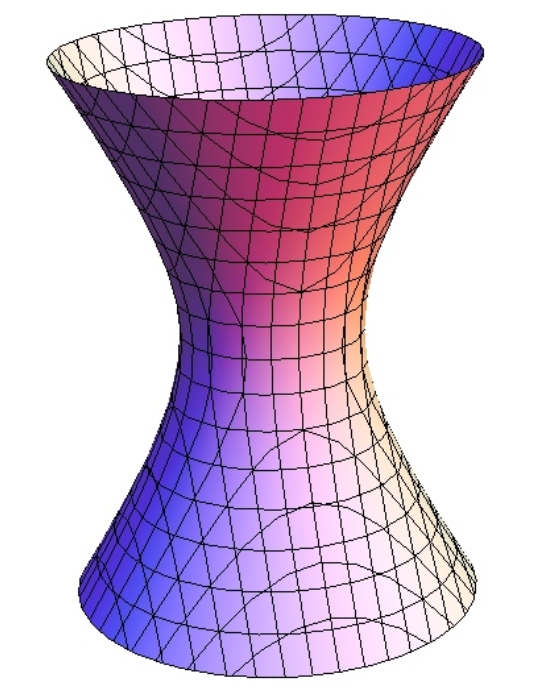
\includegraphics[width=.3\linewidth]{hyperboloid.png}
  \caption{Hyperboloid}
\end{subfigure}%
\begin{subfigure}{.5\textwidth}
  \centering
  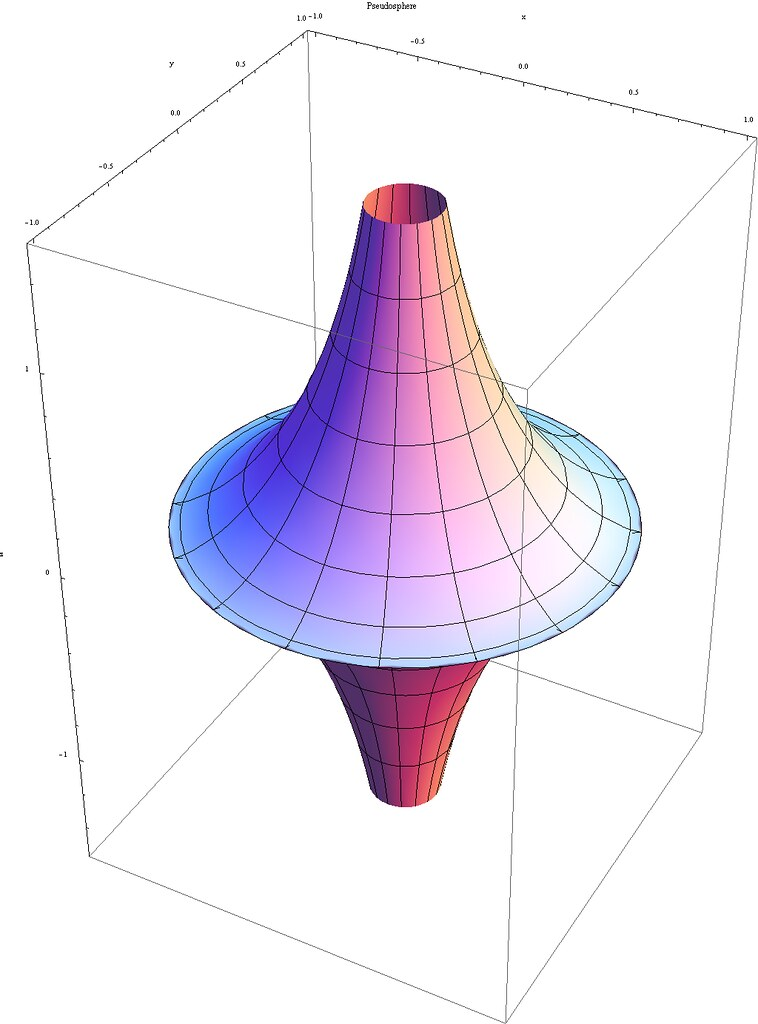
\includegraphics[width=.3\linewidth]{pseudosphere.png}
  \caption{Traktrikoid}
\end{subfigure}
\begin{subfigure}{.5\textwidth}
  \centering
  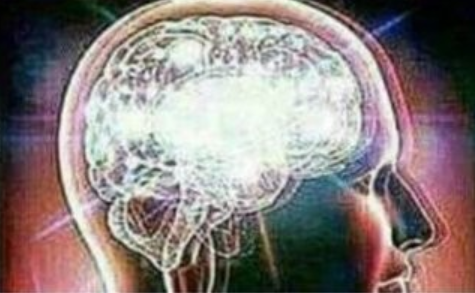
\includegraphics[width=.3\linewidth]{theo_surface.png}
  \caption{theoretische Oberflächen}
\end{subfigure}
\end{figure}

\end{frame}

\begin{frame}{Beispiel: Traktrikoid}

\begin{figure}
\begin{subfigure}{.5\textwidth}
  \centering
  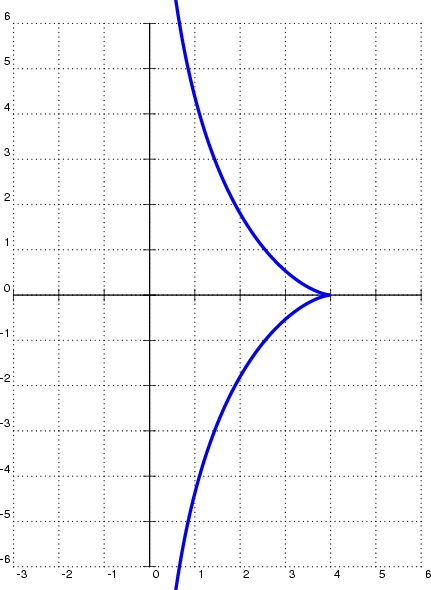
\includegraphics[width=.8\linewidth]{traktrix.png}
  \caption{Traktrix}
\end{subfigure}%
\begin{subfigure}{.5\textwidth}
  \centering
  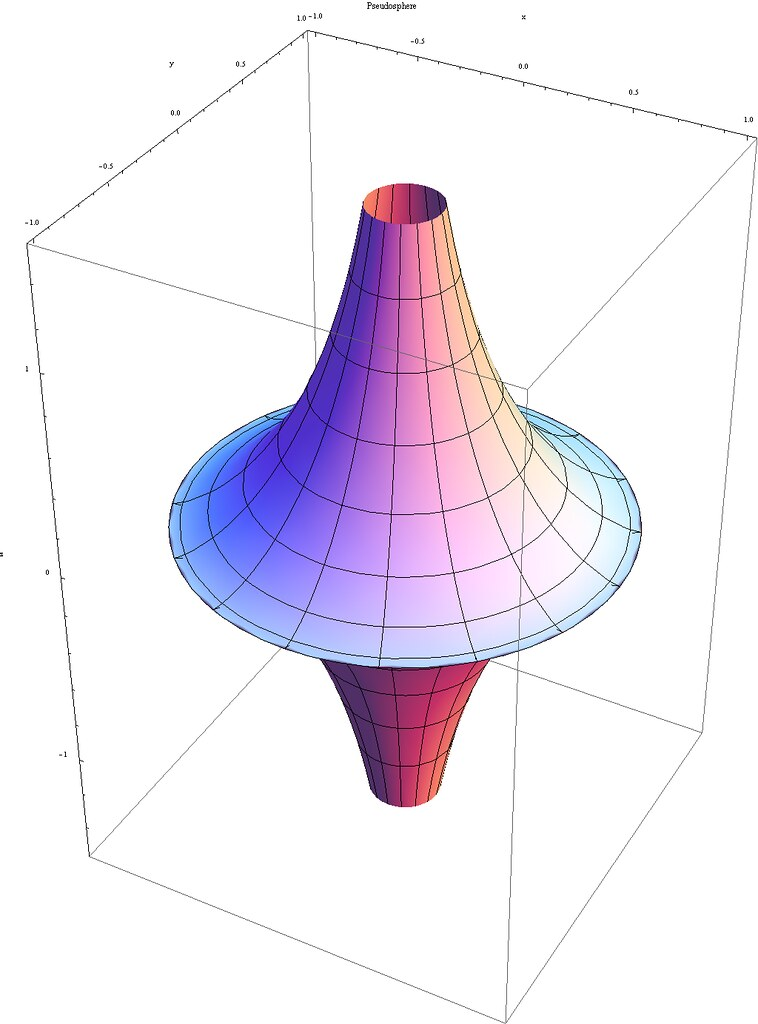
\includegraphics[width=.8\linewidth]{pseudosphere.png}
  \caption{Traktrikoid}
\end{subfigure}

\end{figure}

\end{frame}

\begin{frame}{Definition: Patch}
\begin{mydef}
Ein \textbf{Patch bzw. eine lokale Fläche} ist eine differenzierbare Funktion $x: U \rightarrow \mathbb{R}^n$, mit $U \subset \mathbb{R}^2$ offen. 
\end{mydef}
\end{frame}

\begin{frame}{Definition: Tshebyshev-Patch}
\begin{mydef}
Ein \textbf{Tshebyshev-Patch} mit Radius $a$ ist ein Patch $y: \mathcal{U}\rightarrow \mathbb{R}^n$, dessen Erste Fundamentalform $ds^2 = Edp^2 + 2Fdpdq + Gdq^2$ folgende Eigenschaft besitzt:\newline
$E = G = a^2$
\end{mydef}
\end{frame}

\begin{frame}{Tshebyshev Parametrisierung einer Pseudosphäre}
\begin{mydef}
Sei $a > 0$. Die \textbf{Tshebyshev Parametrisierung} einer Pseudosphäre mit Radius $a$ ist die Abbildung von $\mathbb{R}^2 \rightarrow \mathbb{R}^3$, gegeben durch:
\begin{center}
$(u,v) \mapsto a\Big(\frac{cos(v)}{cosh(u)}, \frac{sin(u)}{cosh(u)}, u - tanh(u)\Big)$.
\end{center}
\end{mydef}
\end{frame}

\begin{frame}{Tshebyshev Parametrisierung einer Pseudosphäre}
\begin{figure}[h!]
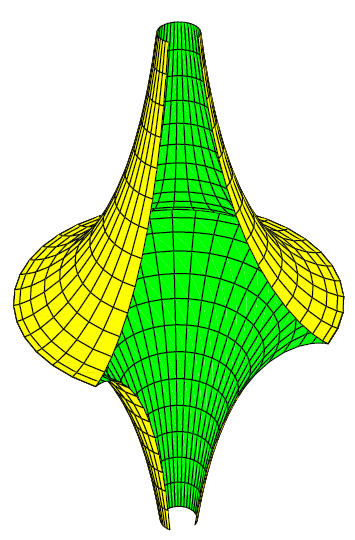
\includegraphics[scale=0.5]{pseudosphere_tchebyshev.png}
\caption{Pseudosphäre nach Tshebyshev Parametrisierung}
\end{figure}
\end{frame}

\begin{frame}{Bianchi - Transformationen}
\begin{mydef}
Sei $\mathcal{M}$ eine Fläche im $\mathbb{R}^3$ mit konstanter Gaußkrümmung $-\frac{1}{a^2}, a > 0$. \newline Eine Fläche $\mathcal{N}$ mit Normalenfeld $U_{\mathcal{N}}$ ist eine \textbf{Bianchi-Transformation} von $\mathcal{M}$, wenn es eine Funktion $\phi : \mathcal{M} \rightarrow \mathcal{N}$ gibt, sodass $\forall p \in \mathcal{M}:$\newline
\begin{itemize}
\item $\norm{\phi (p) - p} = a$
\item $\phi (p) - p$ ist parallel zu einem $v \in T_{p}\mathcal{M}$
\item $U_{\mathcal{N}} (\phi (p))$ ist parallel zu einem $v \in T_{p}\mathcal{M}$ und senkrecht auf $\phi (p) - p$
\end{itemize}
\end{mydef}
\end{frame}

\begin{frame}{Bianchi - Transformationen}
\begin{figure}[h!]
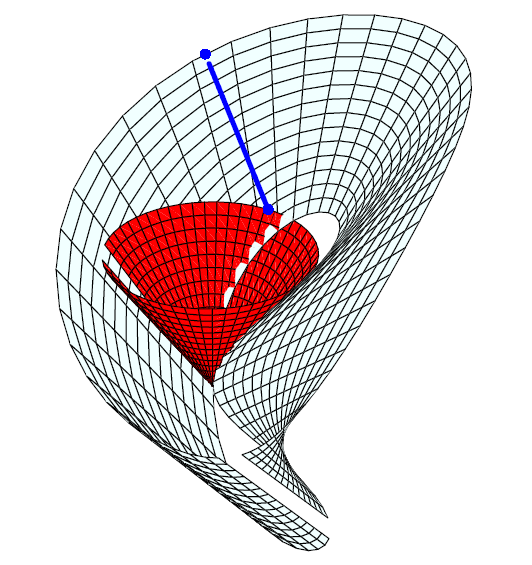
\includegraphics[scale=0.5]{bianchi_transform_def.png}
\caption{Erzeugung einer Fläche durch Translation der Punkte eines runden Kegels}
\end{figure}

\end{frame}

\begin{frame}{Funfact: Erzeugung von Pseudosphären mit Bianchi-Transformationen}
\begin{itemize}
\item wenden Bianchi-Transformation auf den Patch $x(u,v) = (0,0,\epsilon au)$ an, mit $0 < a \equiv const, \epsilon = \pm1$
\item Ergebnis:
\end{itemize}
\centering $\hat{x} = a\Big (\delta cos(v) sech(u), \delta sin(v) sech(u), \epsilon\big(u-tanh(u)\big)\Big)$\newline\newline
$\Rightarrow$ stimmt überein mit dem Patch: \newline\newline
\centering
$(u,v) \mapsto \Big(\frac{a\delta cos(v)}{cosh(u)}, \frac{a\delta sin(v)}{cosh(u)}, a\epsilon\big(u - tanh(u)\big)\Big)$
\end{frame}

\section{Parametrisierung}
\begin{frame}{Kuen'sche Fläche als Bianchi-Transformation der Pseudosphäre}
\begin{mylem}
Sei $\hat{x}$ Bianchi-Transformation der Tshebyshev-Parametrisierung der Pseudosphäre und setze $\theta := 2arctan(e^u)$.
Außerdem sei $\hat{\theta}$ Winkelfunktion von $\hat{x}$. Dann:
\begin{center}
$\hat{\theta}(u,v) = 2arctan\big(-\frac{v}{cosh(u)}\big)$.
\end{center}
\end{mylem}
\end{frame}

\begin{frame}{Kuen'sche Fläche als Bianchi-Transformation der Pseudosphäre}
\begin{mylem}
Wenn $\hat{\theta}$ so ist wie im Lemma gerade, dann:
\begin{tabular}{rl}
&\\
$cos(\hat{\theta})$ & $ = -\frac{v^2 - cosh(u)}{v^2 + cosh^2(u)}$,\\
&\\
$sin(\hat{\theta})$ & $ = \frac{-2v cosh(u)}{v^2 + cosh^2(u)}$
\end{tabular}

\end{mylem}
\end{frame}

\begin{frame}{Kuen'sche Fläche als Bianchi-Transformation der Pseudosphäre}
\begin{mythm}
Die Bianchi-Transformation der Tshebyshev-Parametrisierung der Pseudosphäre ist gegeben durch Gleichsetzen von $\hat{x}$ mit:
\begin{center}
$\Big(\frac{2cosh(u)\big(cos(v) + v sin(v)\big)}{v^2 + cosh^2(u)}, \frac{2cosh(u)\big(sin(v) - v cos(v)\big)}{v^2 + cosh^2(u)}, u - \frac{sinh(2u)}{v^2 + cosh^2(u)}\Big)$
\end{center}
\end{mythm}
\end{frame}

\begin{frame}{Parametrisierung der Kuen'schen Fläche}

\begin{center}
$
\begin{pmatrix}
x\\y\\z
\end{pmatrix}
 =
\begin{pmatrix}
\frac{2cosh(u)* \left( cos(v) + v*sin(v) \right)}{v^2+cosh(u)^2}\\\\
\frac{2cosh(u)*(sin(v) - v*cos(v))}{v^2 + cosh(u)^2}\\\\
u - \frac{sinh(2u)}{v^2 + cosh(u)^2}
\end{pmatrix}
u,v \in \left[ -2\pi , 2\pi \right] $
\end{center}

\end{frame}

\section{Eigenschaften}
\begin{frame}{Eigenschaften der Kuenschen Fläche}
\begin{itemize}
\item Fläche konstanter Gaußkrümmung, aber \textbf{keine} Drehfläche \cite{wuensch}
\item 2-soliton Lösung der Sinus-Gordon-Gleichung \cite{bruter}
\end{itemize}
\end{frame}

\begin{frame}{Sinus-Gordon-Gleichung}
\begin{myeq}
$\phi_{tt} - \phi_{xx} + sin( \phi ) = 0$
\end{myeq}
\textbf{Funfact:}\newline Im 20. Jahrhundert als Modell einer relativistischen Quantenfeldtheorie erneut aufgetaucht\cite{bruter}
\end{frame}

\begin{frame}{Eigenschaften der Kuen'schen Fläche}
\begin{itemize}
\item Fläche konstanter Gaußkrümmung, aber \textbf{keine} Drehfläche \cite{wuensch}
\item 2-soliton Lösung der Sinus-Gordon-Gleichung \cite{bruter}
\item beliebtes Modeaccessoire
\end{itemize}
\end{frame}

\begin{frame}{Kuen'sche Fläche als Statussymbol}
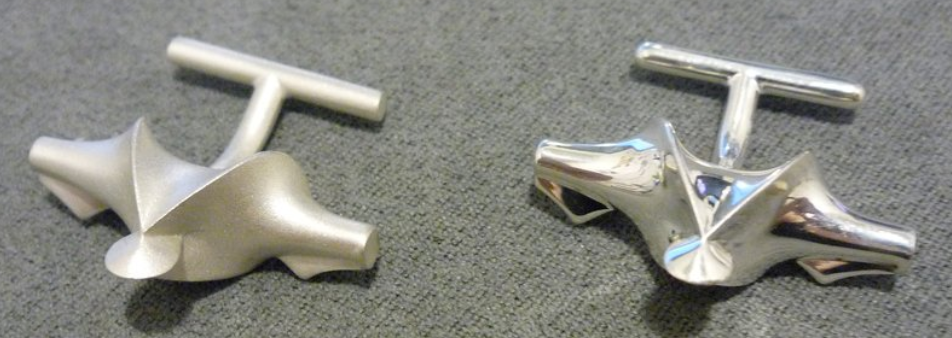
\includegraphics[scale=0.5]{kuen_cuffs.png}
\end{frame}

\begin{frame}{Kuen'sche Fläche als Statussymbol}
\centering
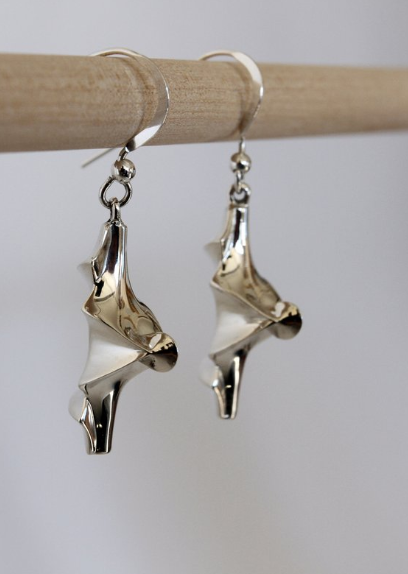
\includegraphics[scale=0.5]{kuen_earrings.png}
\end{frame}

\begin{frame}{Kuen'sche Fläche als Briefbeschwerer}
\centering
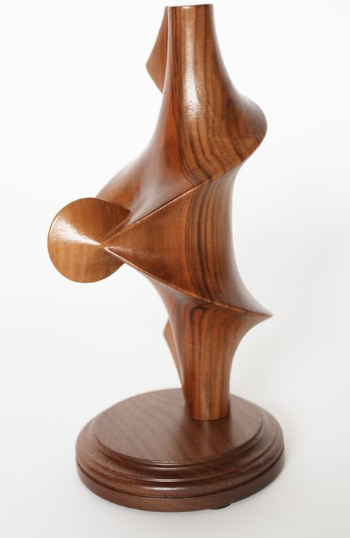
\includegraphics[scale=0.5]{kuen_letter.png}
\end{frame}

\section{Quellen}
\begin{frame}
\footnotesize{
\begin{thebibliography}{99}

\bibitem[Mathcurve] {pseudo_mathcurve} Mathcurve
\newblock The pseudosphere
\newblock \emph{https://www.mathcurve.com/surfaces.gb/\\pseudosphere/pseudosphere.shtml}
\newblock 5. Dezember 2019

\bibitem[Gray] {gray} Modern Differential Geometry of Curves and Surfaces with Mathematica
\newblock Alfred Gray
\newblock 1998

\end{thebibliography}
}

\end{frame}

\begin{frame}
\footnotesize{
\begin{thebibliography}{99}

\bibitem[Scriba] {scriba} 5000 Jahre Geometrie: Geschichte, Kulturen, Menschen
\newblock Christoph Scriba, Peter Schreiber
\newblock Springer Verlag
\newblock 2009

\bibitem[Wünsch] {wuensch} Differentialgeometrie: Kurven und Flächen
\newblock Volkmar Wünsch
\newblock Springer Verlag
\newblock 1997

\end{thebibliography}
}
\end{frame}

\begin{frame}
\footnotesize{
\begin{thebibliography}{99}

\bibitem[Bruter] {bruter} Mathematics and Modern Art
\newblock Claude Bruter
\newblock Springer Verlag
\newblock 2012

\end{thebibliography}
}
\end{frame}

\end{document}